%%%%%%%%%%%%%%%%
\section{Introduction}

\begin{frame}{Introduction}{}
    \begin{figure}[H]
        \centering
        \includegraphics[width=.6\linewidth]{figures/frontpage}
    \end{figure}
    \begin{itemize}
         \item Environmental monitoring
         \item Marine biological research
         \item Bathymetric measurements
         \item Control theory for an ASV
    \end{itemize}
\end{frame}

\begin{frame}{Introduction}{Use Case}
    \begin{figure}[H]
        \centering
        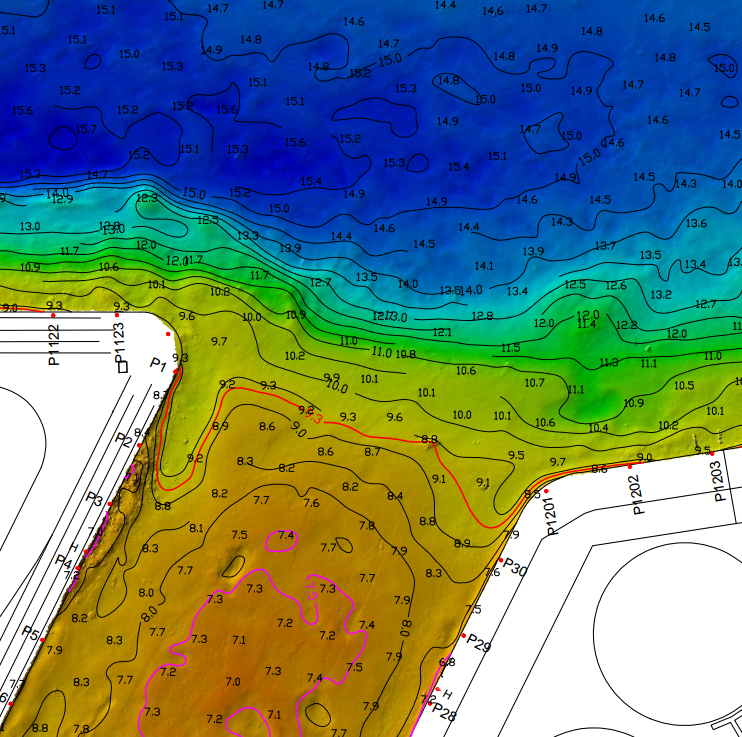
\includegraphics[width=.4\linewidth]{figures/smallDebthMapAalborg}
    \end{figure}
    \begin{itemize}
        \item Depth map used by Port of Aalborg 
        \item Problem: No recent knowledge of depths of the port
        \item Solution: Automate smaller unmanned vessel
    \end{itemize}
\end{frame}

\section{System Description}
\begin{frame}{System Description}{}
    \begin{minipage}{0.45\linewidth}
    \begin{figure}[H]
        \centering
        \includegraphics[width=1\linewidth]{figures/system}
    \end{figure}        
    \end{minipage}\hfill      
    \begin{minipage}{0.45\linewidth}
    \begin{figure}[H]
        \centering
        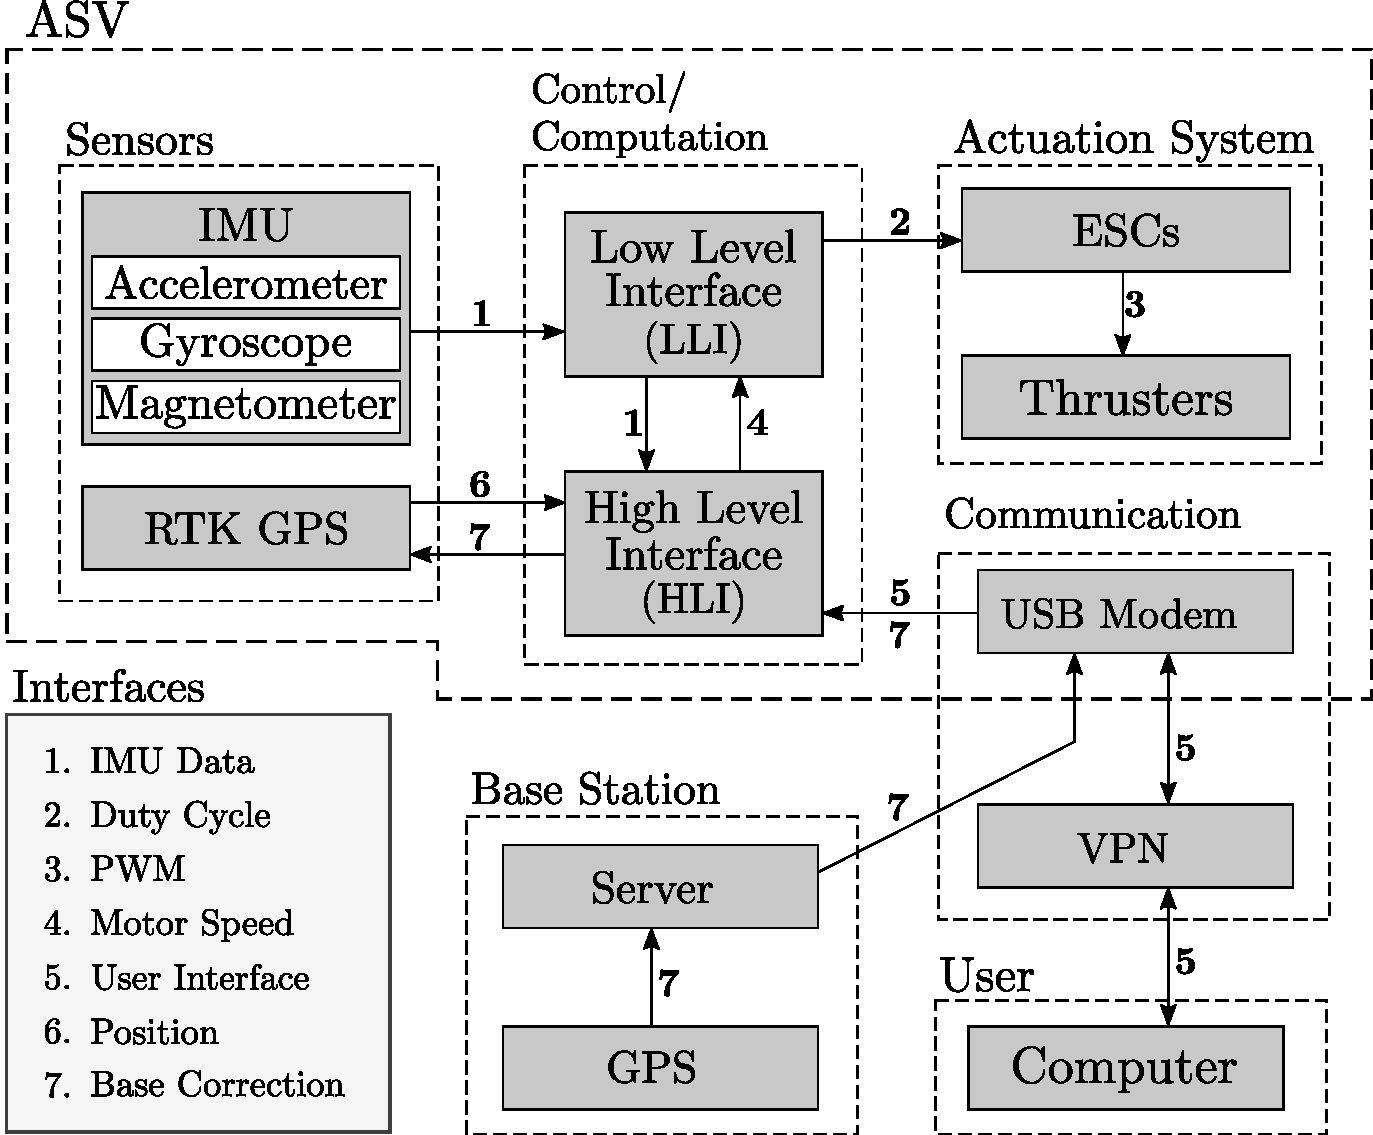
\includegraphics[width=1\linewidth]{figures/systemDiagram5}
    \end{figure}                
    \end{minipage}\hfill \\
\end{frame}

\begin{frame}{System Description}{RTK GPS}
    \begin{figure}[H]
        \centering
        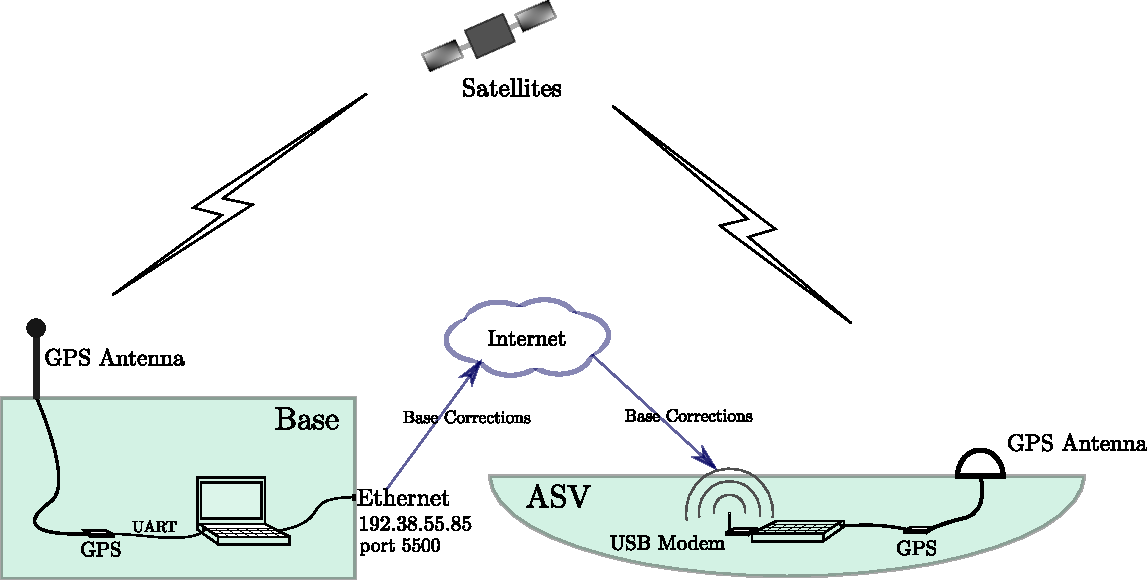
\includegraphics[width=0.7\linewidth]{figures/comunicationSetup}
    \end{figure}        

\end{frame}

%%%%%%%%%%%%%%%%
\section{Model}

%\subsection{Reference Frames}
\begin{frame}{Model}{Reference Frames}
    \begin{figure}[H]
        \centering
        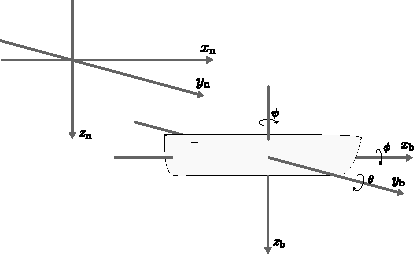
\includegraphics[width=0.7\linewidth]{figures/boat3D}
    \end{figure}
    \begin{itemize}
        \item Inertial Frame (NED)
        \item Body Frame
    \end{itemize}
\end{frame}

%\subsection{Model Dynamics}
\begin{frame}{Model}{Model Dynamics}
    \begin{minipage}{0.5\linewidth}
        \begin{figure}[H]
            \centering
            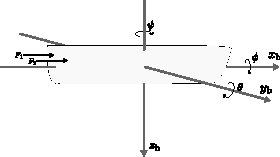
\includegraphics[width=0.8\linewidth]{figures/boat3DForces}
        \end{figure}
        \begin{figure}[H]
            \centering
            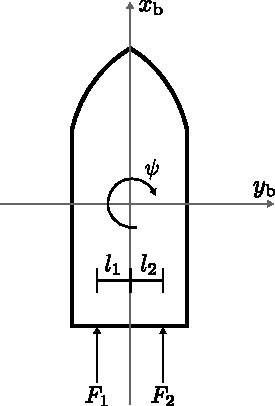
\includegraphics[width=0.4\linewidth]{figures/boat2D}
        \end{figure}         
    \end{minipage}\hfill      
    \begin{minipage}{0.5\linewidth}
        \begin{itemize}
            \item Rigid Body Dynamics
            \begin{flalign}
                \sum F&=m \ddot{x} \nonumber \\
                \sum \tau&=I \ddot{\theta} \nonumber
            \end{flalign}
            \item Hydrostatics
            \begin{itemize}
                \item[-] Buoyancy Force
            \end{itemize}
            \item Hydrodynamics
            \begin{itemize}
                \item[-] Viscous Damping
            \end{itemize}
        \end{itemize}              
    \end{minipage}\hfill \\
\end{frame}

% %\subsection{Rigid Body Dynamics}
% \begin{frame}{Model}{Rigid Body Dynamics}
%     \begin{minipage}{0.65\linewidth}
%         \begin{figure}[H]
%             \centering
%             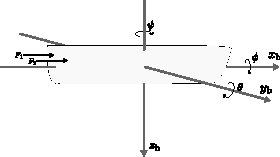
\includegraphics[width=1\linewidth]{figures/boat3DForces}
%         \end{figure}        
%     \end{minipage}\hfill      
%     \begin{minipage}{0.3\linewidth}
%         \begin{figure}[H]
%             \centering
%             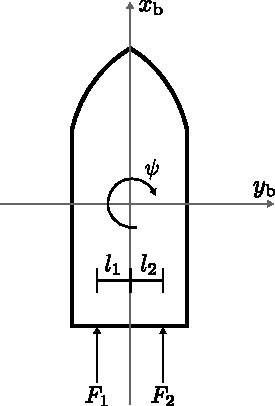
\includegraphics[width=0.7\linewidth]{figures/boat2D}
%         \end{figure}                
%     \end{minipage}\hfill \\
%     \begin{flalign}
%         \sum F&=m \ddot{x} \nonumber \\
%         \sum \tau&=I \ddot{\theta} \nonumber
%     \end{flalign}
% \end{frame}

% %\subsection{Hydrostatics}
% \begin{frame}{Model}{Hydrostatics}
%     \begin{minipage}{0.65\linewidth}
%         \begin{figure}[H]
%             \centering
%             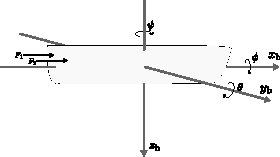
\includegraphics[width=1\linewidth]{figures/boat3DForces}
%         \end{figure}        
%     \end{minipage}\hfill      
%     \begin{minipage}{0.3\linewidth}
%         \begin{figure}[H]
%             \centering
%             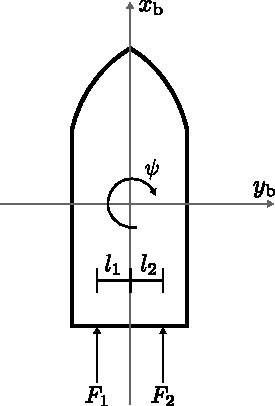
\includegraphics[width=0.7\linewidth]{figures/boat2D}
%         \end{figure}                
%     \end{minipage}\hfill \\
%     \begin{itemize}
%         \item Buoyancy Force
%     \end{itemize}
% \end{frame}

% %\subsection{Hydrodynamics}
% \begin{frame}{Model}{Hydrodynamics}
%     \begin{minipage}{0.65\linewidth}
%         \begin{figure}[H]
%             \centering
%             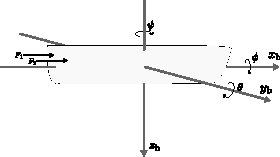
\includegraphics[width=1\linewidth]{figures/boat3DForces}
%         \end{figure}        
%     \end{minipage}\hfill      
%     \begin{minipage}{0.3\linewidth}
%         \begin{figure}[H]
%             \centering
%             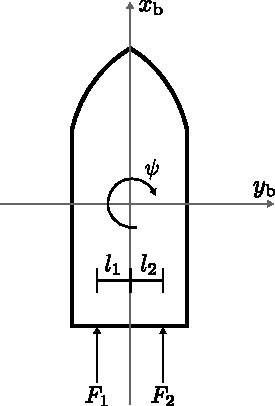
\includegraphics[width=0.7\linewidth]{figures/boat2D}
%         \end{figure}                
%     \end{minipage}\hfill \\
%     \begin{itemize}
%         \item Added mass
%         \item Viscous Damping
%     \end{itemize}
% \end{frame}

%\subsection{Model Equations}
\begin{frame}{Model}{Model Equations}
    \begin{minipage}{0.5\linewidth}
        \begin{figure}[H]
            \centering
            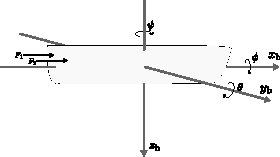
\includegraphics[width=1\linewidth]{figures/boat3DForces}
        \end{figure}        
    \end{minipage}\hfill      
    \begin{minipage}{0.5\linewidth}
        \begin{flalign}
            m \ddot{x}_\mathrm{b} &=  F_\mathrm{1} + F_\mathrm{2}  - d_{\dot{x}_\mathrm{b}} \dot{x}_\mathrm{b} + F_{x_\mathrm{b}}  \nonumber \\
            m \ddot{y}_\mathrm{b} &=  -d_{\dot{y}_\mathrm{b}} \dot{y_\mathrm{b}} + F_{y_\mathrm{b}}  \nonumber \\
            m \ddot{z}_\mathrm{b} &=  -d_{\dot{z}_\mathrm{b}}\dot{z_\mathrm{b}} + F_{z_\mathrm{b}}  \nonumber \\
            I_\mathrm{x}\ddot{\phi} &= -d_{\dot{\phi}} \dot{\phi} + T_\mathrm{\phi}   \nonumber \\
            I_\mathrm{y}\ddot{\theta} &= -d_{\dot{\theta}} \dot{\theta} + T_\mathrm{\theta}   \nonumber \\
            I_\mathrm{z}\ddot{\psi} &= F_\mathrm{1}l_\mathrm{1} - F_\mathrm{2} l_\mathrm{2} - d_{\dot{\psi}} \dot{\psi}  \nonumber
        \end{flalign}              
    \end{minipage}\hfill \\
\end{frame}

%\subsection{Model Equations}
\begin{frame}{Model}{Linearized Model Equations}
    \begin{minipage}{0.5\linewidth}
        \begin{figure}[H]
            \centering
            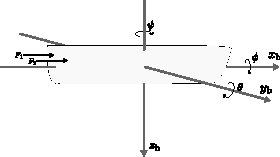
\includegraphics[width=1\linewidth]{figures/boat3DForces}
        \end{figure}        
    \end{minipage}\hfill      
    \begin{minipage}{0.5\linewidth}
        \begin{flalign}
            m \ddot{x}_\mathrm{b} &=  F_\mathrm{1} + F_\mathrm{2}  - d_{\dot{x}_\mathrm{b}} \dot{x}_\mathrm{b} \nonumber \\
            m \ddot{y}_\mathrm{b} &=  -d_{\dot{y}_\mathrm{b}} \dot{y_\mathrm{b}} \nonumber \\
            m \ddot{z}_\mathrm{b} &=  -d_{\dot{z}_\mathrm{b}}\dot{z_\mathrm{b}} -\rho g A_\mathrm{wp} \tilde{z}_\mathrm{n} \nonumber  \\
            I_\mathrm{x}\ddot{\phi} &= -d_{\dot{\phi}} \dot{\phi} - \rho g V \overline{GM_{T}}\cdot \phi \nonumber \\
            I_\mathrm{y}\ddot{\theta} &= -d_{\dot{\theta}} \dot{\theta} - \rho g V \overline{GM_{L}}\cdot \theta \nonumber \\
            I_\mathrm{z}\ddot{\psi} &= F_\mathrm{1}l_\mathrm{1} - F_\mathrm{2} l_\mathrm{2} - d_{\dot{\psi}} \dot{\psi} \nonumber
        \end{flalign}              
    \end{minipage}\hfill \\
\end{frame}

% %\subsection{Model Equations 2}
% \begin{frame}{Model}{Model Equations 2}
%     \begin{minipage}{0.3\linewidth}
%         \begin{figure}[H]
%             \centering
%             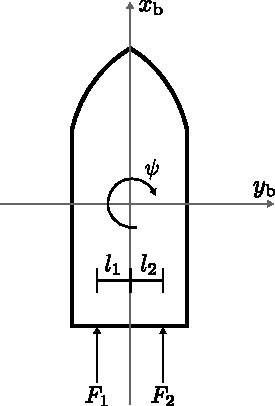
\includegraphics[width=1\linewidth]{figures/boat2D}
%         \end{figure}        
%     \end{minipage}\hfill      
%     \begin{minipage}{0.65\linewidth}
%         \begin{flalign}
%             m \ddot{x}_\mathrm{b} &=  F_\mathrm{1} + F_\mathrm{2}  - d_{\dot{x}_\mathrm{b}} \dot{x}_\mathrm{b} + F_{x_\mathrm{b}}  \nonumber \\
%             m \ddot{y}_\mathrm{b} &=  -d_{\dot{y}_\mathrm{b}} \dot{y_\mathrm{b}} + F_{y_\mathrm{b}}  \nonumber \\
%             m \ddot{z}_\mathrm{b} &=  -d_{\dot{z}_\mathrm{b}}\dot{z_\mathrm{b}} + F_{z_\mathrm{b}}  \nonumber \\
%             I_\mathrm{x}\ddot{\phi} &= -d_{\dot{\phi}} \dot{\phi} + T_\mathrm{\phi}   \nonumber \\
%             I_\mathrm{y}\ddot{\theta} &= -d_{\dot{\theta}} \dot{\theta} + T_\mathrm{\theta}   \nonumber \\
%             I_\mathrm{z}\ddot{\psi} &= F_\mathrm{1}l_\mathrm{1} - F_\mathrm{2} l_\mathrm{2} - d_{\dot{\psi}} \dot{\psi}  \nonumber
%         \end{flalign}              
%     \end{minipage}\hfill \\
% \end{frame}

%\subsection{Model Verification}
\begin{frame}{Model}{Model Verification}
    \begin{itemize}
        \item Verified Nonlinear Model
    \end{itemize}
    \begin{minipage}{0.45\linewidth}
        \begin{figure}[H]
            \centering
            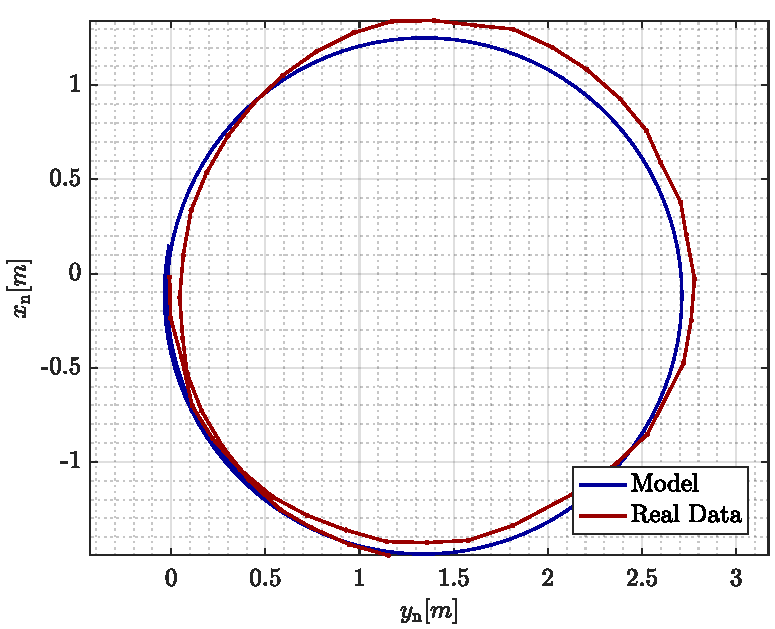
\includegraphics[width=1\linewidth]{figures/turn}
        \end{figure}        
    \end{minipage}\hfill      
    \begin{minipage}{0.45\linewidth}
        \begin{figure}[H]
            \centering
            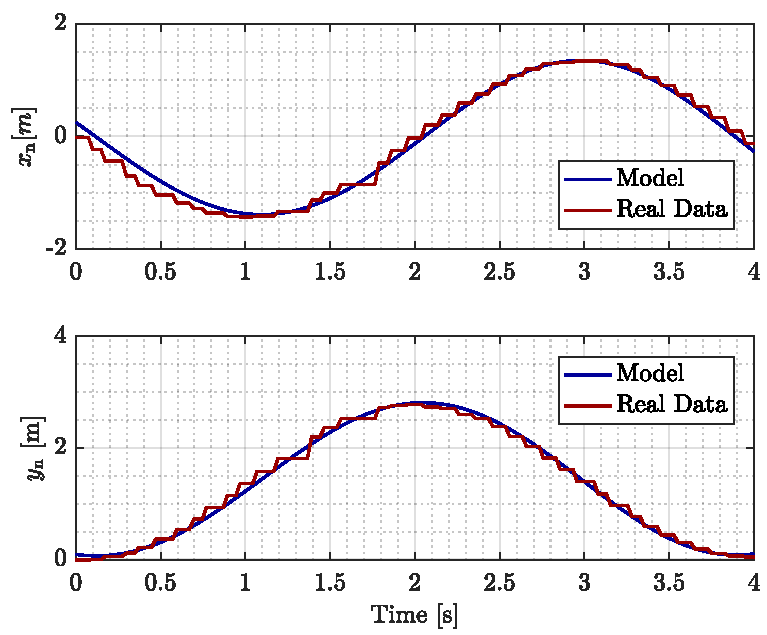
\includegraphics[width=1\linewidth]{figures/turn_time}
        \end{figure}                
    \end{minipage}\hfill \\
\end{frame}






